\question 为了使多个进程能有效地同时处理输入和输出,最好使用( )结构的缓冲技术
\par\twoch{\textcolor{red}{缓冲池}}{循环缓冲}{单缓冲}{双缓冲}
\begin{solution}缓冲池是系统共用资源,可供多个进程共享,并且既能用于输入又能用于输出。其他选项并不能很好地支持多个进程使用。
\end{solution}
\question 为了使并发进程有效输入和输出,应该采用( )结构的缓冲技术
\par\twoch{双缓冲}{环形缓冲}{\textcolor{red}{缓冲池}}{多队列轮转}
\begin{solution}目前计算机系统中广泛使用缓冲池,缓冲池中的缓冲区可供多个进程共享.缓冲池由多个缓冲区组成,其中的缓冲区可供多个进程共享,并且既能用于输入又能用于输出.因此本题应选C。
\end{solution}
\question 下列说法正确的有( )。
Ⅰ.如果I/O所花费的时间比CPU处理时间短的多,则缓冲区最有效
Ⅱ.提高单机资源利用率的最关键技术是SPOOLing技术
Ⅲ.在采用SPOOLing技术的系统中,用户的打印数据首先被送到内存固定区域
Ⅳ.在操作系统中,用户在使用I/O设备时,通常采用物理设备名
\par\twoch{Ⅰ、Ⅲ}{Ⅱ、Ⅲ}{Ⅲ}{\textcolor{red}{都错}}
\begin{solution}Ⅰ错误:缓冲区主要解决I/O速度比CPU处理的速度慢而造成的数据积压的矛盾,所以如果I/O花费的时间比CPU处理时间短的多,则缓冲区就没有必要设置。
Ⅱ错误:在单级系统中,最关键的资源就是处理机资源,最大化地提高处理机利用率,就是最大化地提高系统效率。多道程序设计技术是提高处理机利用率的最关键技术。
Ⅲ错误:打印数据先存入输出井,再送入打印机,输出井位于磁盘而不是内存。
Ⅳ错误:采用的是逻辑设备名,不是物理设备名。 综上所述,本题选择D选项。
\end{solution}
\question 某文件占10个磁盘块,现要把该文件磁盘块逐个读入主存缓冲区,并送用户区进行分析。假设一个缓冲区与一个磁盘块大小相同,把一个磁盘块读入缓冲区的时间为100μs,将缓冲区的数据传送到用户区的时间是50μs,CPU对一块数据进行分析的时间为50μs。在单缓冲区和双缓冲区结构下,读入并分析完该文件的时间分别是(
)
\par\twoch{1500μs,1000μs}{\textcolor{red}{1550μs,1100μs}}{1550μs,1550μs}{2000μs,2000μs}
\begin{solution}见下图:
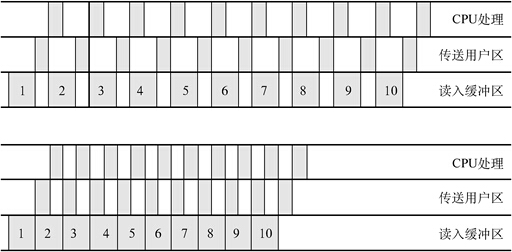
\includegraphics[width=5.33333in,height=2.62500in]{computerassets/a01088e1ad64284318d10c440d72b7f2.jpeg}
图中上半部分为单缓冲,下半部分为双缓冲。每个标号的格子长度为100,没标号的格子长度为50,代表对应处理步骤所需的时间。
在单缓冲的情况下,当上一个磁盘块从缓冲区读入用户区完成时下一磁盘块才能开始读入,将读入缓冲区和传送用户区作为一个单元,共有10个这样的单元,也就是150×10μs=
1500μs,加上最后一个磁盘块的CPU处理时间50μs,得1550μs。
在双缓冲区情况下,读入第一个缓冲区之后可以立即开始读入第二个缓冲区,读完第二个缓冲区之后,第一个缓冲区已经把数据传送至用户区,第一个缓冲区空闲,可以立即开始继续将数据读入第一个缓冲区中,因此不存在等待磁盘块从缓冲区读入用户区的问题,得到传输数据全部传输到缓冲区的时间为100×10μs=1000μs,再加上将最后一个缓冲区的数据传输到用户区并由CPU处理完的时间(50+50)μs=100μs,得1100μs。
【总结】
这种分部处理的缓冲区题目与组成原理中的指令流水线类似,可以通过画图来解决,按照处理步骤分成若干时间轴,将处理步骤画在轴上,可以很直观地看到答案。
\end{solution}
\question 设系统缓冲区和用户工作区均采用单缓冲,从外设读入1个数据块到系统缓冲区的时间为100,从系统缓冲区读入1个数据块到用户工作区的时间为5,对用户工作区中的1个数据块进行分析的时间为90(如下图所示)。进程从外设读入并分析2个数据块的最短时间是(
)。
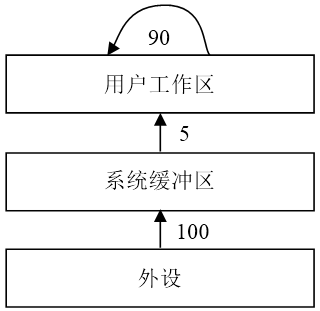
\includegraphics[width=3.33333in,height=3.23958in]{computerassets/815C069B515DDB872D4B79D177AF07B7.png}
\par\twoch{200}{295}{\textcolor{red}{300}}{390}
\begin{solution}数据块1从外设到用户工作区的总时间为105,在这段时间中,系统缓冲区均被数据块1占据,因此对数据块2无法进行操作。但在数据块1在用户工作区进行分析处理时(时间90),系统缓冲区已空闲下来,可以让数据块2从外设读入到系统缓冲区,相当于数据块2的整个处理时间比串行执行时节省了90的时间。又因为数据块串行执行时,第一块所需时间为100+5+90=195,第二块的处理时间为195-90=105,合计195+105=300,即进程从外设读入并分析2个数据块的最短时间为300。
\end{solution}
